Por se tratar de um ambiente de simulação de realidade virtual, alguns parâmetros foram identificados a fim de estabelecer a melhor relação física entre o dispositivo projetado e a verdadeira sensação de um passeio ou corrida de bicicleta. Os sistemas foram desenvolvidos de acordo com os requisitos estabelecidos pelo projeto e posteriormente integrados entre as frentes de controle, estrutura e software presentes no mesmo.

\section{Sistema de Elevação Vertical Dianteiro}

Em um simples passeio de bicicleta é comum lidarmos com situações adversas de terreno, ou seja, variações na declividade em razão a existência de subidas e descidas bem como ainda a existência de planos. O \textit{V-Ride} conta com um sistema de acionamento vertical dianteiro que emula a realidade entendida pelo usuário quando imerso em ambiente de variações de terreno significativas. 

O acionamento figura-se em um princípio básico de ativação: um motor acoplado a um eixo presente em um macaco hidráulico movimenta um parafuso de potência transformando o movimento horizontal linear em movimento vertical linear. Todo princípio de acionamento é controlado pela atuação de um motor, sendo assim, a escolha do mesmo é fundamental para a determinação do correto movimento a ser transmitido, e por conseqüência garantir a movimentação dianteira em concordância a simulação de realidade pretendida. 

Por se tratar de um movimento de caráter sensível e preciso, o projeto \textit{V-Ride} encontrou na modernidade a facilidade no emprego de uma tecnologia consolidada no mercado: o macaco elétrico. A tecnologia viabiliza a operação funcional do sistema de elevação vertical, uma vez que quando  dimensionado,o torque, executado pelo motor é capaz de saciar as necessidade de carga exigidas pelo usuário.

\subsection{Motor Elétrico}

O motor elétrico é um dispositivo que converte energia elétrica em energia mecânica. O mesmo pode ser operado mediante alimentação de corrente contínua ou alternada. O princípio de funcionamento de um motor elétrico se dá pela interação entre campos eletromagnéticos. A existência de uma força mecânica gerada por uma corrente que flui sobre um fio nele presente, quando imerso em um campo magnético, viabiliza e rotação de uma de suas partes, o rotor. 
                
\begin{center}
\includegraphics[scale=0.7]{figuras/rotor}
\captionof{figure}{Componentes de um motor elétrico. Fonte:  Zona da Tecnologia}
\label{rotor}
\end{center}

Principais componentes de um motor elétrico: 

\begin{itemize}
\item 
I.Rotor
\end{itemize}
O rotor é o componente que gira em uma máquina elétrica. Ele é formado por um eixo que abriga um conjunto de bobinas enroladas sobre um núcleo magnético que pode girar sobre um campo magnético criado por um imã ou um conjunto de bobinas presentes no estator.
\begin{itemize}
\item 
II. Estator
\end{itemize}
O estator é a parte fixa do motor e tem por finalidade conduzir o fluxo magnético para rotação do rotor, parte móvel da máquina elétrica. É no estator que é criado um campo magnético capaz de induzir corrente elétrica no conjunto móvel.     

\subsection{Dimensionamento}

Antes de qualquer aplicação prática, um dimensionamento prévio deve ser estabelecido a fim de determinar a escolha do melhor motor para uso. Com isso, um estudo prévio deve ser feito a fim de garantir a funcionalidade e aplicabilidade pretendidas com o uso da máquina elétrica. Alguns parâmetros foram então identificados e determinados como forma de garantir o correto dimensionamento do motor.

\begin{itemize}
\item 
- Análise das forças envolvidas: 
\end{itemize}
                                                          
\begin{center}
\includegraphics[scale=0.7]{figuras/item}
\captionof{figure}{Diagrama de corpo livre do macaco hidráulico}
\label{item}
\end{center}

O valor do ângulo beta presente na figura foi obtido previamente com valor aproximado de 20$^{\circ}$ . Aplicando o somatório de forças atuante sobre o braço superior direito, temos:

\[\sum Fy= 0\]

\[- \frac{P}{2} + F1\times  sen \beta  =  0\]

\[F1 = \frac{P}{2} \times sen \beta\]

Considerando que o usuário, bicicleta e a mesa giratória presente na parte dianteira possuem peso aproximado de 1300 N, temos: 

\[F1 = 1900,47 N\]

Para a determinação de aplicação sobre o fuso do macaco, aplicamos o somatório das forças no eixo x, então: 

\[\sum Fx= 0\]

\[- 2 \times F1 \times cos \beta + F2 = 0 \]

\[F2 = 2 \times F1 \times cos \beta\]

   Aplicando o valor de F1 encontrado no item anterior encontramos o valor da força axial máxima quando \ss é o valor aproximado do ângulo determinado: 

\[F2 = 2 \times 1900,47  \times cos 20 \degree \]

\[F2 = 3571,71 N\] 

    Assim temos que a carga axial máxima no fuso no momento do levantamento é de 3571,71 N. Os braços sofrem ação de uma força de compressão e nas piores condições sustentam uma força de 1900,47 N.
Considerando que o usuário, bicicleta e a mesa giratória presente na parte dianteira possuem peso aproximado de 1300 N, temos: 

\[F1 = 1900,47 N\]

Para a determinação de aplicação sobre o fuso do macaco, aplicamos o somatório das forças no eixo x, então: 

Velocidade máxima desempenhada pelo motor: 

A partir das especificações técnicas do motor presente no macaco elétrico, o cálculo da velocidade máxima de levantamento para a carga nominal foi calculado: 

\begin{center}
    \includegraphics[scale=0.7]{figuras/calculado}
       \captionof{figure}{ Tabela 1. Especificações técnicas do motor elétrico}
       \label{calculado}
   \end{center}   

A potência útil desempenhada pelo motor deve ser calcula usando: 

\[Pot útil = \eta \times Pot\]

Sabendo que \eta é o coeficiente de performance da caixa de redução presente no equipamento, e seu valor variando entre faixa de 94\% à 97\%, temos: 

\[Pot útil = 0,97 \times 100\]

\[Pot útil = 97 W\]                          

   Potência mecânica é definida pela equação abaixo, onde \textit{v  } é a velocidade desempenhada pelo motor no levantamento:  

\[Pot útil = F \times \textit{v  } \]

\[\textit{v} = \frac{P útil}{m\times a} \] 

A partir da eq. 3, e considerando que a massa total é a massa do conjunto usuário, bicicleta e mesa tendo valor igual a 130 Kg e a aceleração da gravidade igual 10 m/s2 : 

\[\textit{v} = \frac{97}{130 \times 10}\]  
   
\[\textit{v} = 0,07446 m/s\]

Definindo a velocidade linear em função da freqüência de rotação do motor a partir da equação 6, onde r é o raio de do eixo do motor: 

\[\textit{v} = 2 \times \pi \times r \times \textit{f  } \]       

\[0,07446 = 2 \times \pi \times 0,006 \times \textit{f  } \]   

\[\textit{f} = 0,07446/0,03769\]

\[\textit{f} = 1,975 Hz\] 

Determinando o número de rotações por minuto basta multiplicarmos a freqüência de operação por 60, uma vez que a freqüência é o número de ciclos por segundo: 

\[\textit{f}  = 118,5 RPM\]
                
Dessa forma, o motor produz aproximadamente 119 rotações por minuto quando operado em velocidade nominal para a carga total associada. Esse parâmetro é variável, uma vez que a carga total é função do usuário e do peso da bicicleta acoplada no sistema. 

\section{Sistema de Alimentação de Energia }

O conceito de sustentabilidade está cada vez mais imerso no dia a dia do ser humano. A ideia de tornar sustentável e a capacidade de reutilização tornam-se obséquio da capacidade humana em desenvolver maneiras ainda mais versáteis e inovadoras em detrimento à dependência por tecnologias já consolidadas e de alto custo de manutenção. Com isso, o projeto \textit{V-Ride} conta com um sistema próprio de geração de energia elétrica a partir do movimento mecânico gerado pelas pedaladas do usuário.

O circuito será responsável por fornecer carga a bateria de um celular quando necessitado pelo usuário durante o uso do \textit{V-Ride}. Uma fonte geradora, dínamo, é responsável pela conversão mecânica das pedaladas imprimidas pelo usuário em corrente elétrica que alimenta a bateria.

\subsection{Circuito carregador rede elétrica}  

O circuito integrado ao circuito gerador tem por fonte a rede elétrica residencial. Sabendo que a tensão da bateria utilizada para armazenamento da energia elétrica apresenta tensão inferior a tensão fornecida pela rede, foi necessário a construção de um carregador que atendesse aos parâmetros de carregamento da bateria.

O dispositivo capaz de interagir com os valores disponibilizados pela rede é o transformador. Assim, o grupo adequou-se ao uso do componente que é capaz de receber uma alta tensão, oriunda da rede elétrica, e disponibilizasse a tensão de recarga indicada pelo fabricante da bateria. Por se tratar de fontes de natureza distintas, ou seja, a rede elétrica disponibiliza corrente alternada e a bateria é alimentada por corrente contínua, criou-se a necessidade de retificação da corrente de saída do transformador. A ponte retificadora consiste em configuração de diodos em ponte, ou ponte de “Wheatstone”, capaz de ‘linearizar’ o sinal oscilatório de natureza alternada.
                            
        
\begin{center}
\includegraphics[scale=0.7]{figuras/alternada}
\captionof{figure}{Esboço simplificado carregador de bateria. Fonte: Ebah}
\label{alternada}
\end{center}

Inicialmente é possível identificarmos a presença do transformador. No primário, a tensão de entrada é de 220V, referente a rede; no secundário saída de 15V. A corrente de operação na saída do transformador é de 3A. Com a ponte retificadora o sinal entra alternado e tem saída contínuo. Em 3 é possível identificar a presença de um capacitor, o mesmo é responsável pela filtração do sinal de saída da ponte retificadora, uma vez que a retificação é de onda completa. A necessidade de incremento do banco de capacitores ao circuito se da uni e exclusivamente em razão a otimização e qualidade da corrente que será disponibilizada a bateria.     
                                         
  \begin{center}
    \includegraphics[scale=0.7]{figuras/bateria}
       \captionof{figure}{Ponte retificadora 10A. Fonte: Proesi}
       \label{bateria}
   \end{center}
                                            
\begin{center}
    \includegraphics[scale=0.7]{figuras/trafo}
       \captionof{figure}{Transformador 220V/15V. Fonte: AliExpress}
       \label{trafo}
   \end{center}
                           
                                       
 \begin{center}
    \includegraphics[scale=0.7]{figuras/capacitor}
       \captionof{figure}{Capacitor 2200\[µF\].Fonte: Bau da Eletronica}
       \label{capacitor}
   \end{center}

 
A montagem do circuito carregador foi feito segundo a figura abaixo.         
\begin{center}
    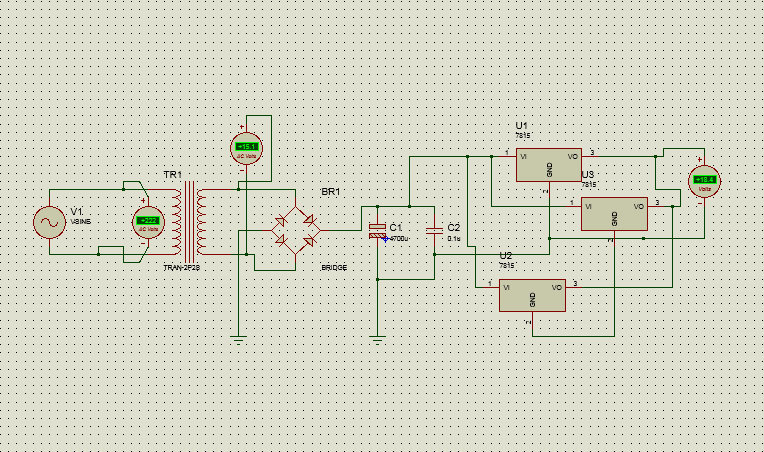
\includegraphics[scale=0.7]{figuras/Fonte-15V}
       \captionof{figure}{ Simulação do circuito do carregador }
       \label{Fonte.15V}
   \end{center}

A representação é feita pela simulação do circuito carregador utilizando o software Proteus. Nela é possível analisarmos uma tensão de 15V na saída do transformador. Após a retificação da corrente, foi conectado em parelelo três reguladores de tensão 7815/1A a fim de dividir a corrente quando exigida em valor máximo pela bateria. A medição do amperímetro indicou valor referente a 18,4V ,a margem é aceitável, uma vez que é superior à tensão da bateria, mas não é o valor ideal, visto que o fabricante determina os valores ótimos para recarga.

\section{Bateria}  

A presença de uma bateria no projeto é justificada pela necessidade de armazenamento da energia proveniente da rede. Sua implementação é justificada pela capacidade de fornecer altos valores de corrente instantânea e também atuando como \textit{no break} para o projeto. A utilização da mesma viabiliza o aproveitamento do usuário por tempo finito quando energia oriunda da rede elétrica não encontra-se disponível. A implementação da mesma  mantem  as melhores condições de funcionamento de equipamentos presentes no projeto, como por exemplo os motores que atuam nos sistemas de elevação e de frenagem.

A fim de  manter  as melhores condições de funcionamento de equipamentos presentes no projeto, como por exemplo os motores que atuam nos sistemas de elevação e de frenagem,o projeto \textit{V-Ride}adequou-se a necessidade do uso de uma bateria que atendesse a simples sistemas de potência, como a operação de motores. Assim, por ser alimentada por uma fonte oriunda da rede, o primeiro passo consiste em escolher uma bateria que apresente tensão inferior a suas formas de alimentação. O passo seguinte é adequar o fornecimento de corrente elétrica necessária a correta alimentação das cargas envolvidas. A figura abaixo ilustra o tipo de bateria utilizada no projeto.

Como sistema complementar, o dínamo empregado para a geração de energia pode operar fornecendo sua energia diretamente a um dispositivo \textit{smartphone} ou ainda para a bateria, dependendo apenas das necessidades criadas pelo usuário.
                                    
                     
\begin{center}
    \includegraphics[scale=0.7]{figuras/bateria}
    \captionof{figure}{ Bateria Moura 12MVA-7 . Fonte: Mercado Livre }
    \label{projeto}
\end{center}
  
Analisando todos os tipos de bateria existentes no mercado e as necessidades geradas pelos equipamentos consumidores de potência elétrica, determinou-se o uso da bateria cuja especificações estão listadas na seguinte tabela

\begin{center}
        \includegraphics[scale=0.7]{figuras/tabela}
       \captionof{figure}{ Bateria Moura 12MVA-7 . Fonte: Mercado Livre }
    \label{tabela}
\end{center}

Os valores apresentados pela tabela são específicos ao tipo de bateria usado no projeto V-Ride. Podemos observar que a mesma possui uma autonomia fixa de 84Wh, ou seja, é capaz de fornecer uma potência constante de 84W por um período fixo de uma hora, suficiente e necessário para alimentação dos componentes elétricos presentes.
Observamos que a mesma apresenta tensão de recarga entre os valores 14,4 V e 14,7 V, ou seja, por apresentar um sistema de alimentação oriundo da rede fora necessário adequação dos sistema de recarga ao uso de um regulador de tensão capaz de manter a tensão nos terminais de entrada da bateria dentro dos valores próximos ao determinado pelo fabricante. 

\section{Sistema de frenagem } 
 
A fim de garantir as melhores condições de simulação da realidade proposta ao usuário, o V-Ride conta com um sistema que emula as condições de terreno impostas. Ou seja, em ambientes de aclividade, a sensação de um pedalar mais difícil é sentida. Tal impressão só é sentida devido a existência de um sistema sensível capaz de operar nas condições de realidade proposta.

Para isso, o acionamento é feito mediante atuação de um motor que acoplado a uma haste de ferro tracionada viabiliza o contato por atrito com uma polia presente no eixo do rolo da estrutura traseira. Por se tratar de um movimento muito preciso e sensível, a transmissão do movimento do motor para a haste deve ocorrer de maneira controlada e gradual, uma vez que o espaço percorrido até o contato é pequeno. O motor que melhor atende as condições necessárias é o motor de passo, capaz de trabalhar com pequenas variações dentro de um passo ou ainda micro passo. 

\subsection{Motor de Passo }  

O motor de passo é um motor elétrico usado em situações onde se deseja obter um posicionamento preciso ou ainda o rotacionamento de um ângulo exato. A rotação desenvolvida pelo motor é controlada por uma série de campos magnéticos emitidos eletronicamente por pulsos ou passos. Por não usar escovas ou comutadores, o motor possui um número fixo de pólos magnéticos que determinam o número de passos por revolução executada.  O número de passos realizados executa a variação de um certo ângulo rotacionado pelo eixo do motor, sendo o controle desses passos realizado de maneira computacional e uma das formas mais versáteis de sistema de posicionamento. 

\subsection{Especificações do Motor de Passo } 
 
O motor de passo utilizado no sistema de frenagem apresenta as especifiações listadas segundo a figura 9 abaixo:                       
\begin{center}
    \includegraphics[scale=0.7]{figuras/tec}
       \captionof{figure}{ Dados técnicos motor de passo   }
       \label{tec}
   \end{center}

O torque de manutenção apresentado é de 5,2kgf. cm .Para as necessidades criadas o valor é superior, entretanto por ser uma máquina que estava disponível para uso apenas houve a adequação da mesma ao funcionamento do sistema de frenagem. 

Outro parâmetro considerável para análise de dimensionamento do motor é a faixa de freqüência de operação e o torque por ele produzido. Tendo em vista que o mesmo irá operar dentro de um curto período de tempo, o mesmo é capaz de satisfazer os valores entendidos para carga durante ambientes de inclinação.

Por se tratar de uma máquina que apresenta movimento controlado e sensível, o motor de passo requer um sistema responsável pelo seu controle. Assim, criou-se a necessidade de conexão de um driver ao motor. O grupo estabeleceu os parâmetros necessitados e com isso desenvolveu o próprio driver do motor  que será explicitado mais detalhadamente em subtópico seguinte.       
      
\begin{center}
    \includegraphics[scale=0.7]{figuras/torque}
       \captionof{figure}{ Curva Torque x Frequência de operação}
       \label{toque}
   \end{center}

\subsection{Geração de Energia }  
Uma máquina elétrica nada mais é que um dispositivo que realiza a conversão entre energia mecânica e energia elétrica, quando esta conversão é feita no sentido da transformação da energia mecânica em energia elétrica esta máquina recebe o nome de gerador, esta conversão normalmente ocorre devido a atuação de um campo magnético \cite{chapp2000}.
Para o escopo deste trabalho decidiu-se utilizar um alternador com o objetivo de converter a energia mecânica oriunda das pedaladas do usuário na bicicleta em energia elétrica para alimentar os componentes da solução.

As duas principais partes das máquinas elétricas são o estator e o rotor, o estator consiste em um conjunto de órgãos ligados rigidamente à carcaça, que possui bobinas com enrolamentos e o rotor é sistema rígido que gira em torno de um eixo apoiado em mancais fixos na carcaça, que é constituído por por dois núcleos polares (polos magnéticos Norte e Sul),  uma bobina indutora, dois anéis coletores e um veio \cite{neto2000}.

Sendo assim, podemos destacar ainda que nestas máquinas teremos um indutor que será responsável por produzir o campo magnético, e o induzido que receberá a corrente induzida, então no alternador o rotor faz o papel de indutor, enquanto o estator fará o papel de induzido, assim como a conversão obedecerá o princípio da Lei de Lenz, pois uma corrente induzida produzirá um campo magnético que por sua vez exercerá forças contrárias a rotação do rotor, isto explica a necessidade do rotor nestas máquinas elétricas demandarem acionamento mecânico \cite{neto2000}.

Inicialmente decidiu-se por utilizar um alternador automotivo, uma vez que o mesmo atendia os requisitos de aplicação impostos pelo projeto e já possuía integrado os sistemas de retificação, regulação de tensão e proteção contra correntes reversas, as principais partes do alternador automotivo são descritos a seguir:

\begin{center}
    \includegraphics[scale=0.7]{figuras/partes}
       \captionof{figure}{  Partes de um Alternador. Fonte: General Motors}
       \label{partes}
   \end{center}

Como posse das supracitadas informações foi decidido por utilizar um Alternador da marca Bosh 14 V 80 A/h que foi acoplado ao rolo de treino da estrutura por uma correia que liga a polia do alternador a uma polia que foi instalada no rolo, da seguinte forma:


\begin{center}
    \includegraphics[scale=0.7]{figuras/alt}
       \captionof{figure}{  Alternador acoplado ao rolo de treino.}
       \label{alt}
   \end{center}

O esquema mostrado acima foi acoplado a uma bateria para serem realizados os testes de validação da solução, com o auxílio de um multímetro foi medida a corrente entre o sistema alternador/bateria. 

O alternador escolhido tem a especificação de mínima rotação para acioná-lo, sendo esta em torno de 800 RPM, no esquema montado têm-se que a relação da roda para da bicicleta para o rolo é de 6:1 e da polia do rolo para a polia do alternador de 2:1, assim sendo estipulou-se que a rotação mínima para acionar a geração de energia é de 67 RPM, o que é um valor razoável que até um usuário sedentário poderia atingir. 

Porém verificou-se experimentalmente que para as condições previstas teoricamente o alternador não era capaz de carregar a bateria uma vez que a corrente obtida na medição era negativa, ou seja o alternador não só não stava cumpindo sua função de carregar a bateria como estava puxando energia da mesma, através de revisão bibliográfica explica-se este fato devido aos componentes citados anteriormente que poderiam vir a demandar energia, assim sendo foram realizados testes em períodos maiores de tempo e variando o sistema de marchas da bicicleta. 

Averigou-se então que em marchas mais pesadas a corrente medida passava a ser positiva e aumentava gradualmente com o aumento da velocidade das pedaladas, porém a solução foi invalidada uma vez que um dos escopos do projeto é propor uma solução modular independente da bicicleta, o que não seria possível devido a dependência da marcha, foram levantadas soluções alternativas, como o aumento da relação entre as polias para causar um efeito multiplicador, porém isto causaria o mesmo efeito do aumento da marcha, ou seja o aumento da sensação de peso pelo usuário, assim sendo, só seria possível gerar energia em um sistema com marcha pesada o que inviabilizaria a simulação de cenários de descida, que é um dos propósitos do jogo. 

Como a utilização do alternador não era mais uma solução viável optou-se por utilizar dínamos de bicicleta, que possuem capacidade de produção de energia bem menos significativas, porém são adaptáveis a todos os requisitos do projeto, além de um sistema com um circuito complementar que permitirá carregar a bateria com o sistema convencional de energia elétrica oriunda da rede para suprir as possíveis demandas que o dínamo não é capaz de atender.

O dínamo que será utilizado é o seguinte:

\begin{center}
    \includegraphics[scale=0.7]{figuras/dinamo}
       \captionof{figure}{  Dínamo a ser usado.}
       \label{dinamo}
   \end{center}

O critério para a seleção do mesmo foi a necessidade que o mesmo possuísse uma tensão superior a tensão da bateria de qualquer celular. Sabe-se que a tensão presente em baterias eletrolíticas presentes nos atuais smartphones são de 5V, e pelo gerador ser uma fonte de fornecimento 16V foi necessário a regulação da tensão a fim de satisfazer as necessidades de carga.O único modelo comercial que possuía estas especificações é o da figura que possui tensão de 16 V e potência máxima de 8 W, como sabe-se que esta potência depende das rotações oriundas da pedaladas vê-se que esta é uma solução proposta apenas para aproveitar a energia mecânica que está sendo gerada. 

Inicialmente o grupo entendeu a viabilizar recarga à bateria por um sistema de alimentação misto, oriundo da rede e da energia gerada pelo dínamo, operando mediante sinais gerados pela detecção do microcomputador a tensão presente na mesma. Por estar sempre conectada em uma fonte de recarga, os sinais de tensão estariam sempre em valores ótimos, inviabilizando o contato por chaveamento entre as fontes de alimentação, assim tal solução fora descartada.   

O circuito carregador consiste então em um dispositivo capaz de fornecer energia mínima para recarga de um celular comum quando demandado pelo usuário. A saída do dínamo é em formas de pulsos, ou seja, demanda retificação para conectá-la a bateria que demanda corrente contínua. A primeira parte da retificação ocorre por meio de uma ponte de diodos em H, os diodos inicialmente usados para teste foram o 1N4004, para a filtragem é utilizado um capacitor de 4700uF que será responsável por diminuir esta pulsação, porém como visto na imagem acima a onda ainda não é completamente linear, então ocorre a estabilização através de um diodo Zenner. Sabendo que a potência do gerador é de 8W com tensão de saída de 8V, o fornecimento de corrente elétrica se da na faixa de 1,5 A, valor capaz de satisfazer as necessidades de carga nominal da bateria. A figura abaixo mostra a representação esquemática e a simulação do circuito do carregador de bateria:

   \begin{center}
        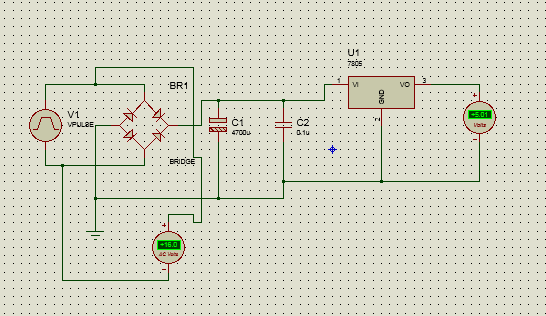
\includegraphics[scale=0.7]{figuras/Fonte-5V}
    \captionof{figure}{Circuito carregador de celular}
    \label{Fonte.5V}
\end{center}

A saída do dínamo é em formas de pulsos, ou seja demanda retificação para conectá-la a bateria que demanda corrente contínua, para tanto será utilizado um circuito retificador como o seguinte: 


\begin{center}
    \includegraphics[scale=0.7]{figuras/ret}
       \captionof{figure}{Circuito a ser implementado em conjunto com o dínamo.}
       \label{ret}
   \end{center}

A primeira parte da retificação ocorre por meio de uma ponte de diodos em H, os diodos inicialmente usados para teste foram o 1N4004, para a filtragem é utilizado um capacitor de 4700uF que será responsável por diminuir esta pulsação, porém como visto na imagem acima a onda ainda não é completamente linear, então ocorre a estabilização através de um diodo Zenner que ainda terá a função de evitar correntes reversas que poderiam a vir da bateria para os dínamos. 

\section{Confecção das Placas de Circuito Impresso}

Os Circuitos Impressos são estruturas onde se fixam componentes eletrônicos, isto ocorre em uma placa de material isolante, este material está sempre na fórmula de lâmina e pode ser feito a partir de diferentes materiais, tais como fenolite, fibra de vidro, materiais cerâmicos em geral  e compósitos que são fabricados a fibra de vidro e a resina fenólica %[7].

A placa laminada é coberta com uma (ou mais) camadas de cobre, neste cobre são desenhadas as trilhas com uma tinta anticorrosiva que pode ser obtida por marcador permanente ou jatos de impressora a laser, em seguida é necessário transferir o layout do circuito, podem ser utilizadas diversas técnicas para realizar isto tais como processo de transferência térmica, processo de transferência fotográfica, processo de transferência serigráfica e fresagem. 

Com as trilhas fixadas na camada de cobre a placa é então submetida ao processo de corrosão, onde todo o cobre que não estiver recoberto com a tinta será degradado, para realizar este processo utiliza-se soluções com propriedades de corrosão do cobre, tais como percloreto de ferro ou persulfato de amônia.   

Em seguida a placa fica coberta pelo cobre somente na parte da trilha, com o auxílio de um perfurador os locais para as conexões são furados e os componentes são soldados com uma solda de linha eutética de chumbo e estanho. 

\subsection{Procedimentos Experimentais da Confecção das Placas de Circuito Impresso}

Foram confeccionadas 3 Placas de Circuito Impresso, a referente ao driver do motor de passo que controla o freio, a referente ao driver do motor de elevação vertical e a referente a placa dos sensores de monitoramento da bicicleta. 

Com o Layout das trilhas condutoras concluído no software Proteus, a imagem foi espelhada e impressa em uma impressora a laser em papel couchê 90 g. 

A técnica escolhida foi realizar o processo de transferência térmica, a placa foi lixada com o auxílio de uma esponja de aço e o papel foi colocado o papel sobre a placa de fenolite (para as PCB’s do driver) e sobre a placa de compósito (para a PCB dos sensores de monitoramento da bicicleta), então foi aplicada pressão e temperatura por aproximadamente 5 minutos, por meio de um ferro de passar.

O resultado obtido foi o seguinte: 

\begin{center}
    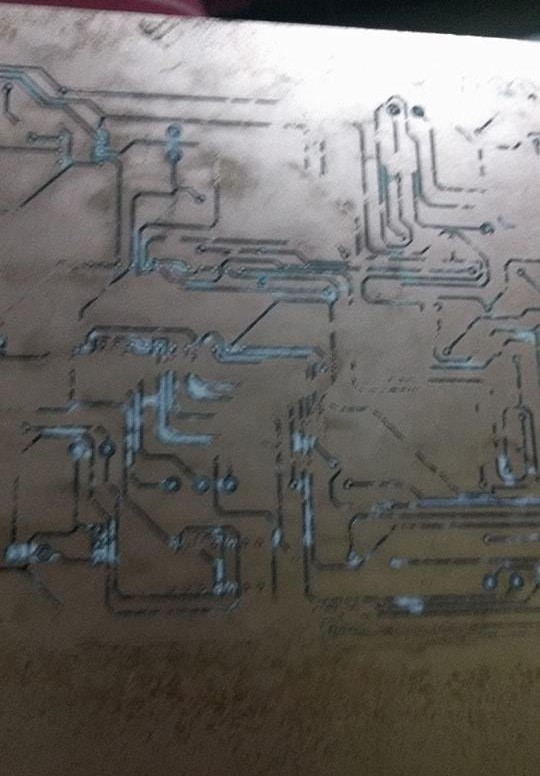
\includegraphics[scale=0.3]{figuras/errada}
       \captionof{figure}{ Tentativa 1 de confecção da PCB dos sensores de monitoramento da bicicleta. }
       \label{errada}
   \end{center}  

Como pode ser observado, o processo não resultou em uma transferência uniforme das trilhas nem possibilitou a total remoção do papel, assim sendo, optou-se por trocar o  papel utilizado e repetir o procedimento, foram realizadas tentativas utilizando papel couchê de 120g, papel fotográfico glossy e papel fotográfico high glossy, todos resultando em resultados falhos e impossibilitando a aplicação. 
Após algumas tentativas optou-se por utilizar o papel etiqueta, de forma que a parte com a etiqueta foi retirada e utilizado o papel residual, isto favoreceu a transferência pois neste papel ficam resíduos de cola da etiqueta, que quando submetidos ao calor facilitam a transferência da tinta para a placa, utilizando este papel e aplicando pressão e temperatura por meio do ferro por aproximadamente 7 minutos foi obtido o seguinte resultado:

\begin{center}
    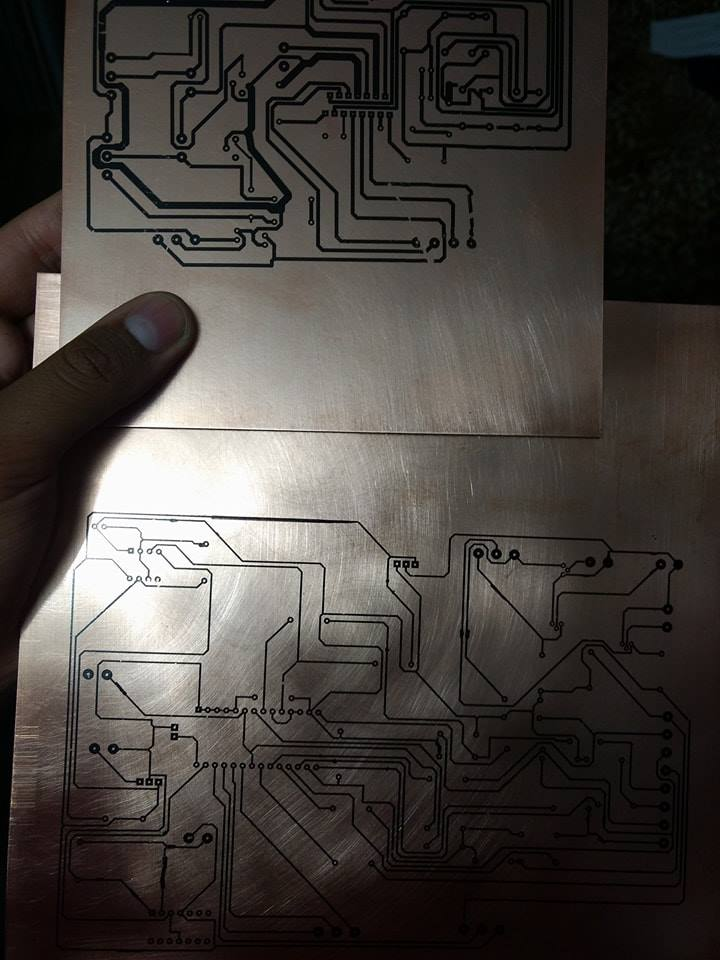
\includegraphics[scale=0.3]{figuras/tinta}
       \captionof{figure}{PCB’s do driver dos motores e da placa dos sensores monitoramento da bicicleta após processo de transferência térmica. }
\label{tinta}
   \end{center}

As pequenas falhas nas trilhas foram cobertas com o auxílio de um marcador permanente, foi realizado um furo na placa, por onde foi passado um pedaço de tecido com o objetivo de permitir a manipulação da placa quando submetida a corrosão, sem que tenha-se contato com a solução. 

A solução escolhida para a realizar o processo de corrosão foi o percloreto de ferro ( FeCl3 ), em um recipiente de plástico foi colocado 1 litro de água e adicionadas 400 g de percloreto de ferro em pó, em seguida a placa foi mergulhada nesta solução por aproximadamente 4 minutos. 

\begin{center}
    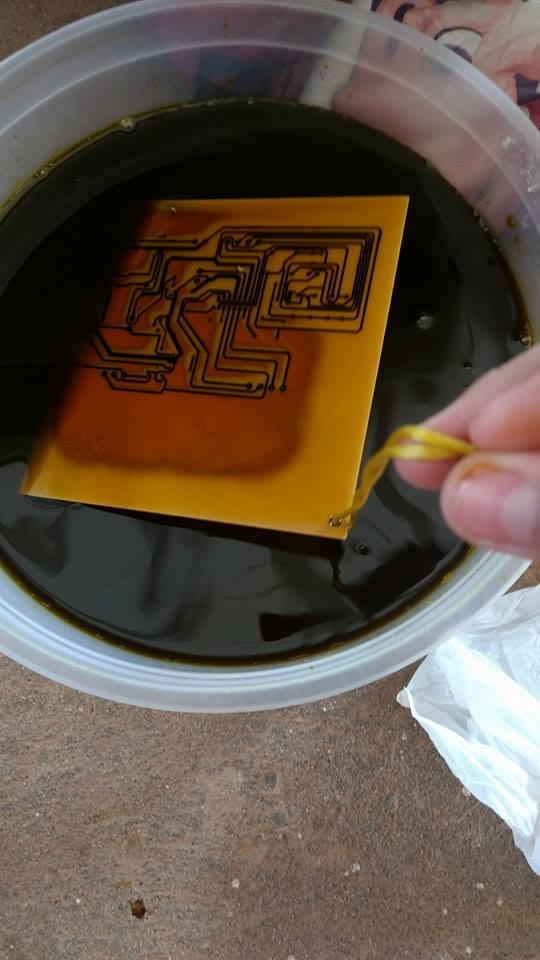
\includegraphics[scale=0.3]{figuras/corroer}
       \captionof{figure}{PCB’s sendo submetidas a processo de corrosão em percloreto de ferro. }
       \label{corroer}
   \end{center}  
Após o processo de corrosão as placas foram novamente limpas com palha de aço para remover a tinta e deixar apenas a trilha condutora de ferro. 
\begin{center}
    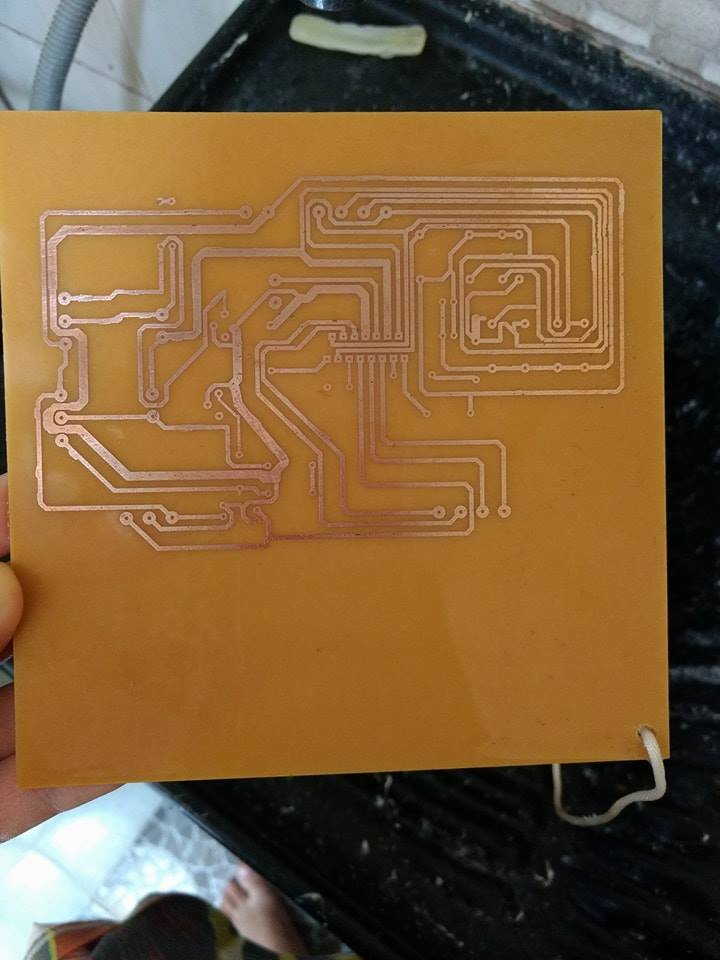
\includegraphics[scale=0.3]{figuras/pronta}
       \captionof{figure}{PCB’s do driver dos motores e da placa dos sensores monitoramento da bicicleta após processo de transferência térmica. }
       \label{pronta}
  \end{center}  
Em seguida, com o auxílio de um perfurador foram realizados os furos para inserir os componentes eletrônicos. 
\begin{center}
    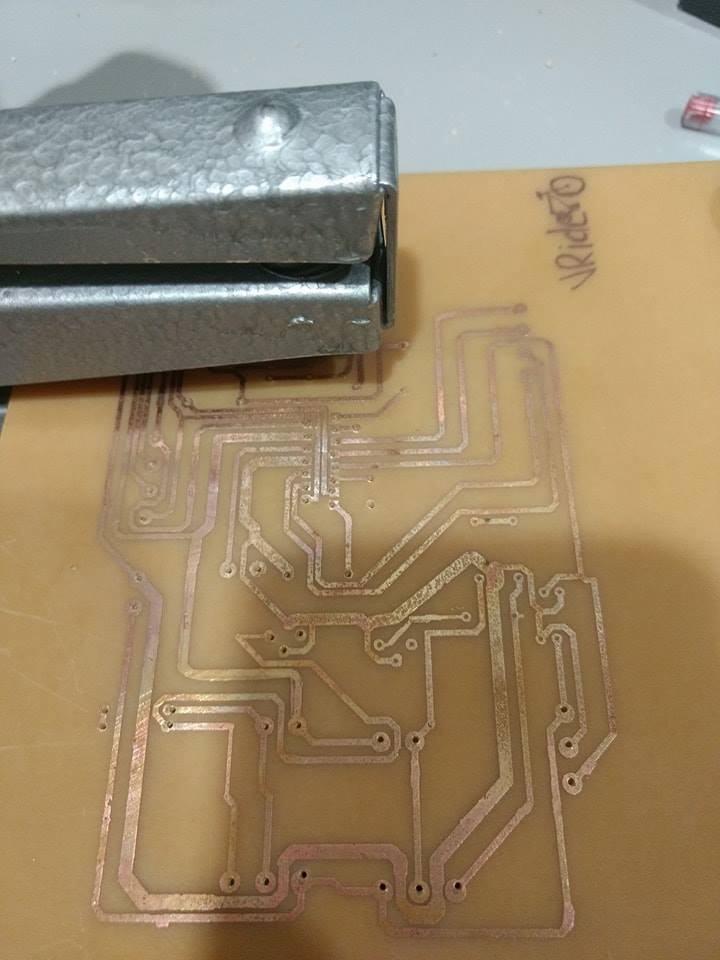
\includegraphics[scale=0.3]{figuras/perfurar}
       \captionof{figure}{PCB’s do driver dos motores e da placa dos sensores monitoramento da bicicleta sendo submetidas a perfuração. }
       \label{perfurar}
  \end{center}  
Por fim, os componentes eletrônicos foram soldados a placa. 
\begin{center}
    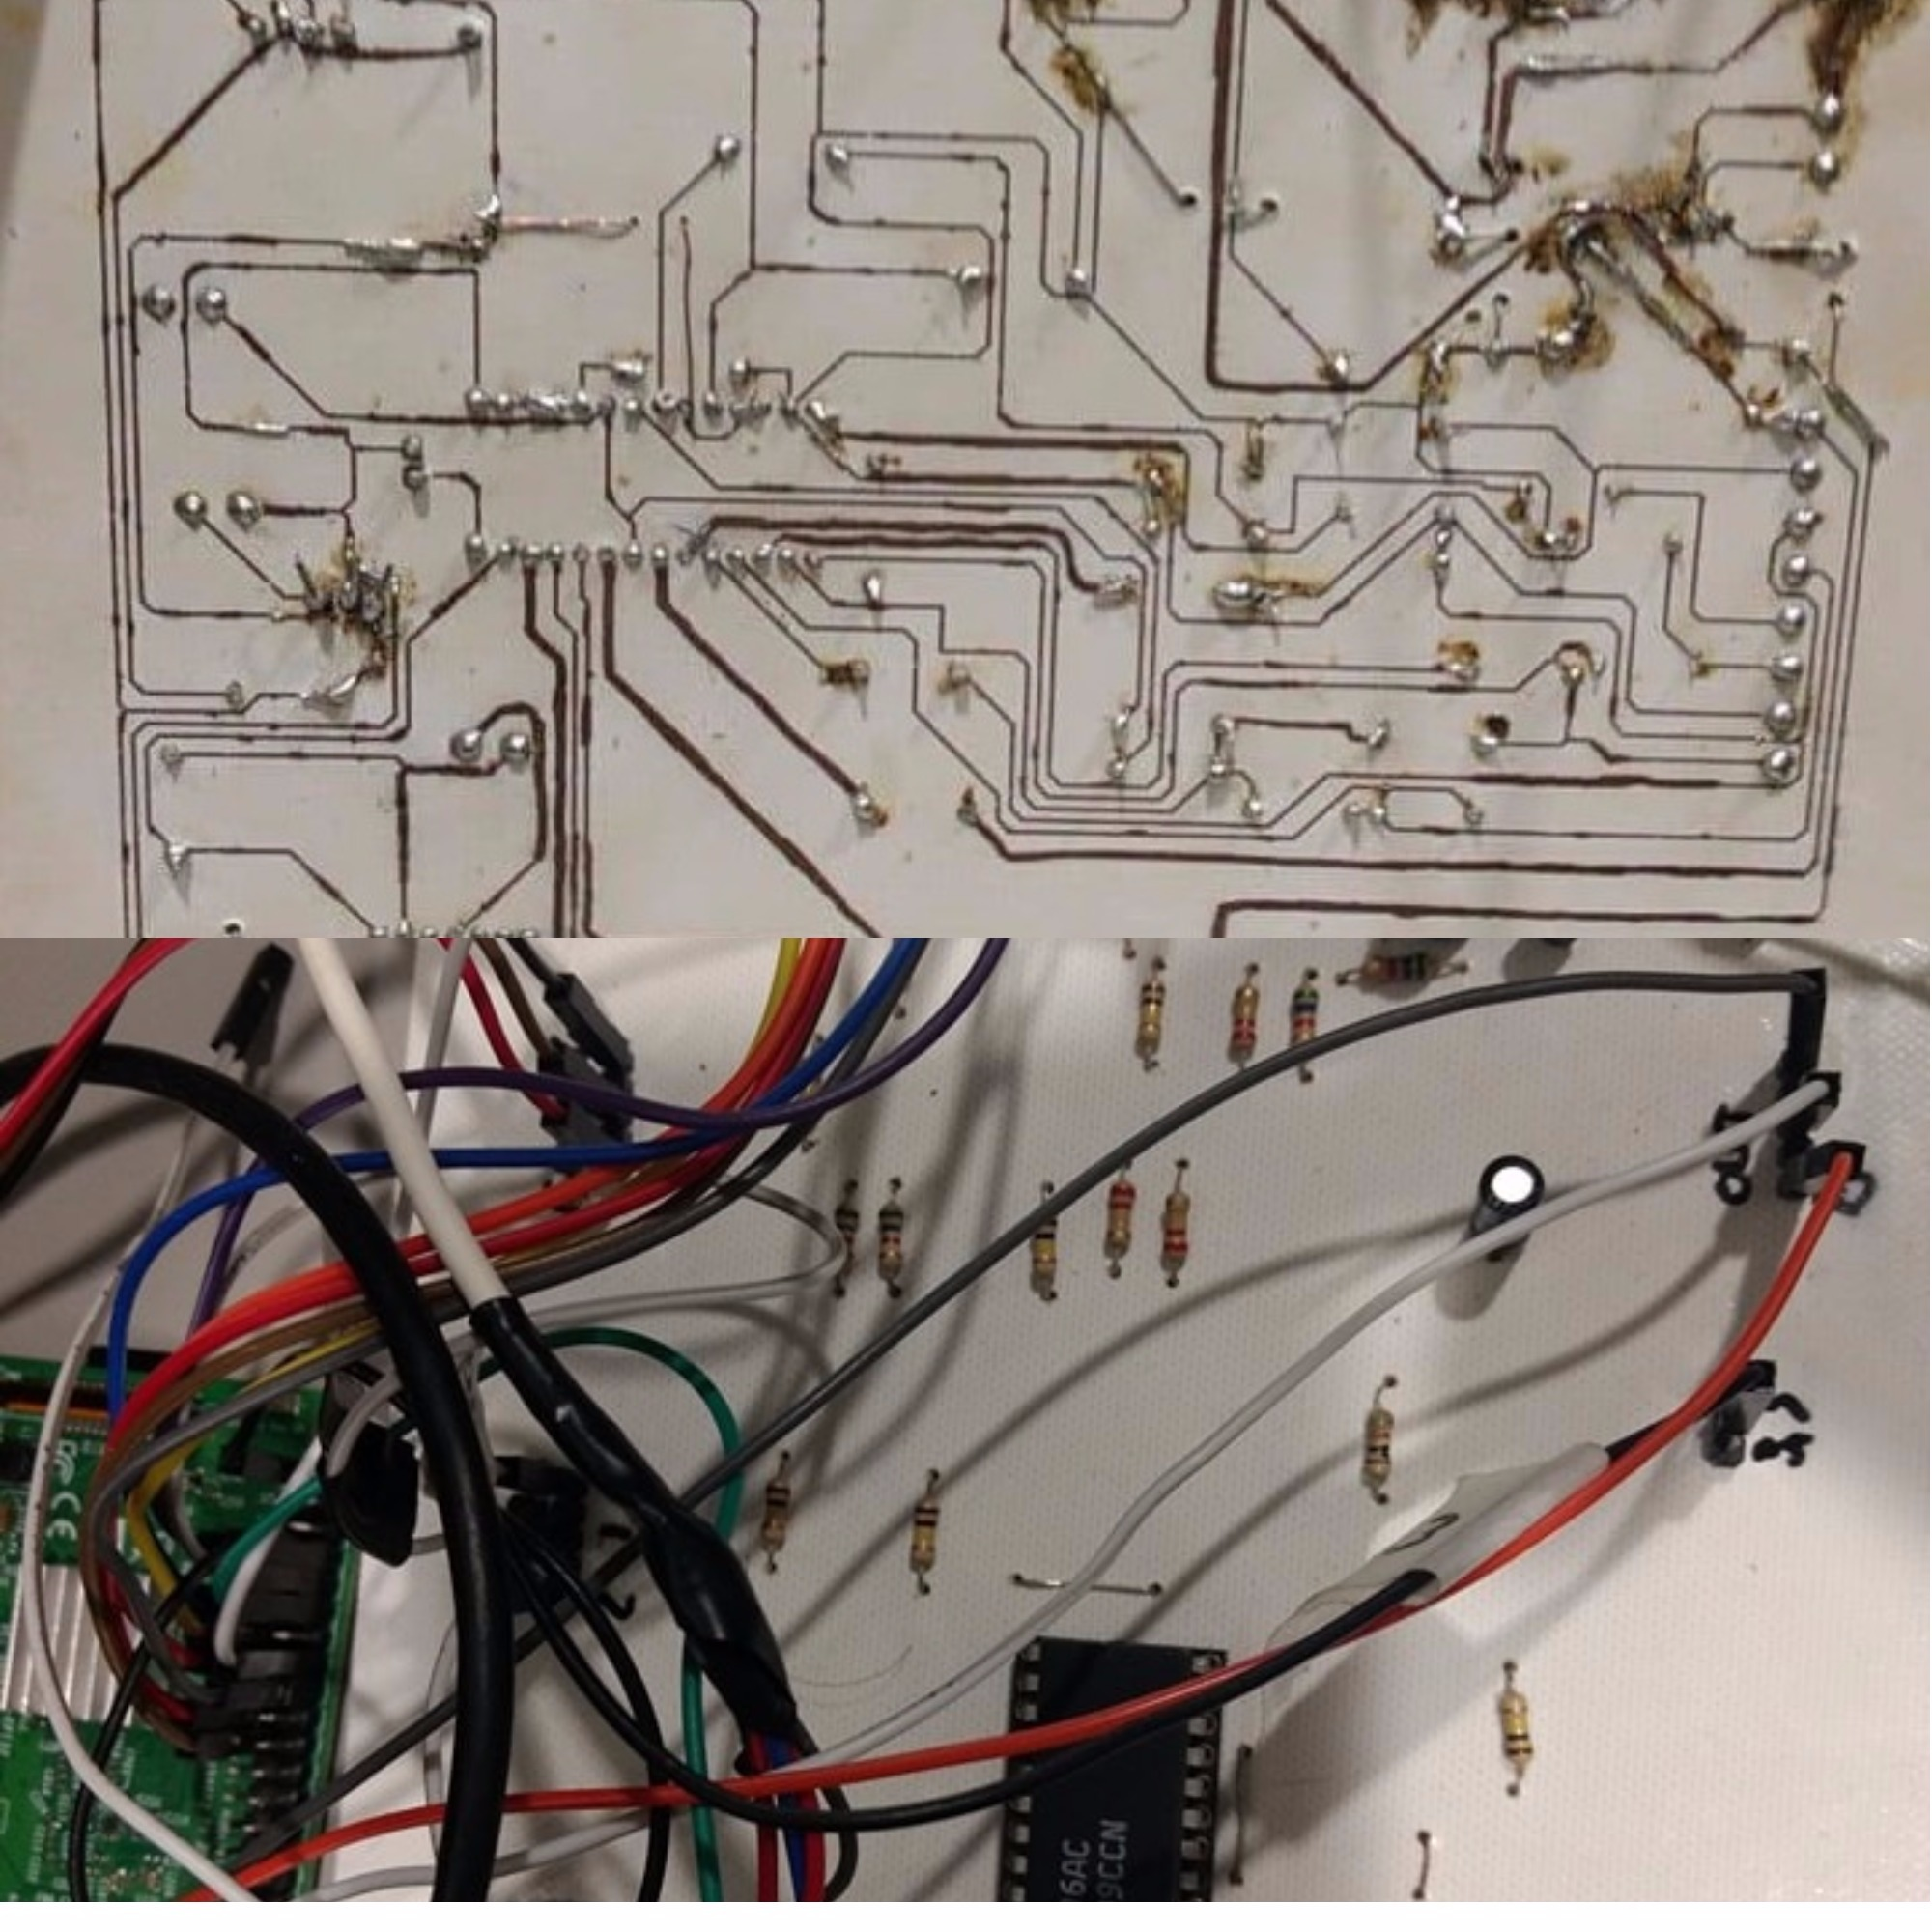
\includegraphics[scale=0.1]{figuras/placa}
       \captionof{figure}{PCB pronta da placa dos sensores monitoramento da bicicleta.}
       \label{placa}
  \end{center}  
\begin{center}
    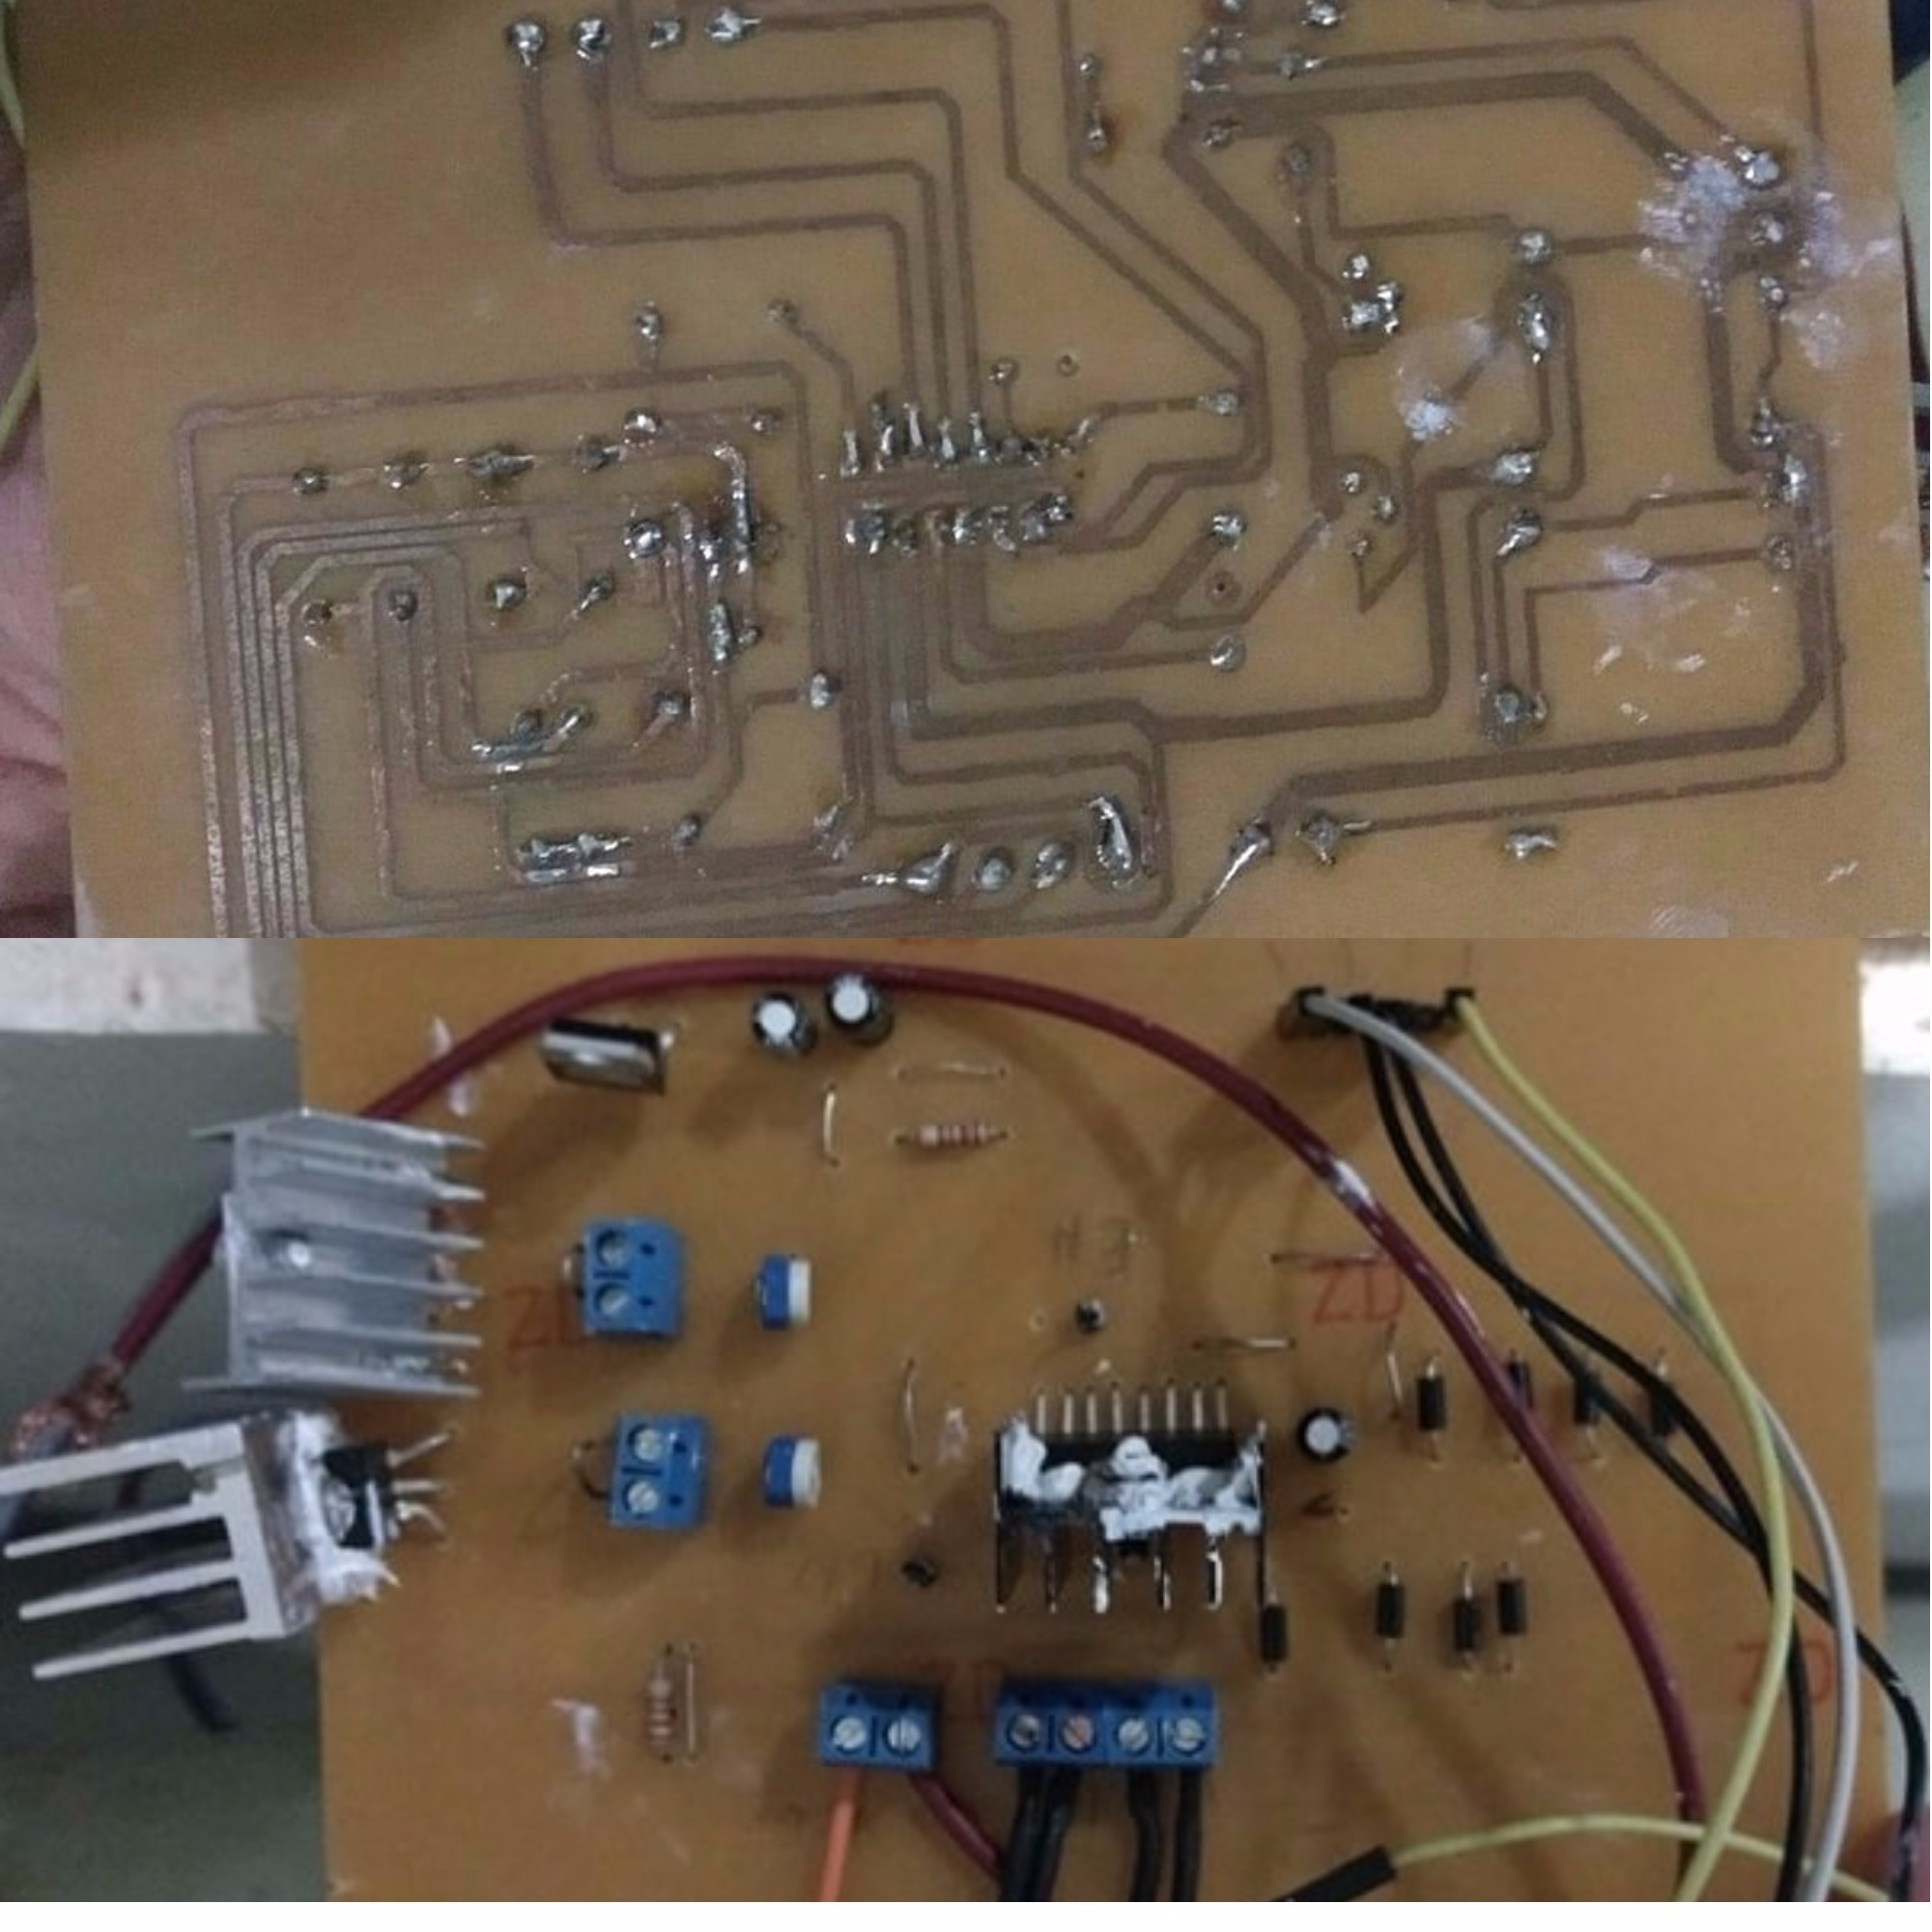
\includegraphics[scale=0.1]{figuras/driver}
       \captionof{figure}{PCB’s dos drivers dos motores.}
       \label{driver}
  \end{center} 


%[1]MARTINS, Lucas Felipe Sarti; MARQUES, Bruno dos Santos; SANTOS, Everton Luiz dos. Desenvolvimento de dispositivo para levantamento de veículos leves e de fácil operação. 2014. 14 f. TCC (Graduação) - Curso de Engenharia Mecanica, Centro Tecnologico, Centro Universitário Católico Salesiano Auxilium, Araçatuba, 2014.

%[2]GALDINO, Luciano. Calculo da Rotação, Torque e da Potencia de motores elétricos para a transmissão por parafuso de potência. 2014. 17 f. Monografia (Especialização) - Curso de Física, Centro Tecnologico, Usp, São Paulo, 2014.

%[3]Chapman, S. J. Fundamentos de Máquinas Elétricas – 5a edição, McGraw-Hill.
%[4]NETTO, L.F. Geradores de Energia Elétrica Disponível em:< http://www.ceee.com.br/pportal/ceee/Component/Controller.aspx?CC=3332>
%[5]General Motors, http://www.gmev.com/evsite/go/specs.htm, EUA, 1997
%[6]CORRADI, J. Circuitos Retificadores. Disponível em: < http://www.corradi.junior.nom.br/Projetosbasicos.pdf>

%[7] JUNIOR, S.S.H; MOURA, F.P.; CORREA, R.S.; AFONSO, J.C.; VIANNA, C.A.; MANTOVANO, J.L. Processamento de placas de circuito impresso de equipamentos eletroeletrônicos de pequeno porte. Disponível em: http://www.scielo.br/scielo.php?script=sci_arttext&pid=S0100-40422013000400015